\documentclass{ximera}

%\usepackage{todonotes}

\newcommand{\todo}{}

\usepackage{esint} % for \oiint
\ifxake%%https://math.meta.stackexchange.com/questions/9973/how-do-you-render-a-closed-surface-double-integral
\renewcommand{\oiint}{{\large\bigcirc}\kern-1.56em\iint}
\fi


\graphicspath{
  {./}
  {ximeraTutorial/}
  {basicPhilosophy/}
  {functionsOfSeveralVariables/}
  {normalVectors/}
  {lagrangeMultipliers/}
  {vectorFields/}
  {greensTheorem/}
  {shapeOfThingsToCome/}
  {dotProducts/}
  {partialDerivativesAndTheGradientVector/}
  {../productAndQuotientRules/exercises/}
  {../normalVectors/exercisesParametricPlots/}
  {../continuityOfFunctionsOfSeveralVariables/exercises/}
  {../partialDerivativesAndTheGradientVector/exercises/}
  {../directionalDerivativeAndChainRule/exercises/}
  {../commonCoordinates/exercisesCylindricalCoordinates/}
  {../commonCoordinates/exercisesSphericalCoordinates/}
  {../greensTheorem/exercisesCurlAndLineIntegrals/}
  {../greensTheorem/exercisesDivergenceAndLineIntegrals/}
  {../shapeOfThingsToCome/exercisesDivergenceTheorem/}
  {../greensTheorem/}
  {../shapeOfThingsToCome/}
  {../separableDifferentialEquations/exercises/}
  {vectorFields/}
}

\newcommand{\mooculus}{\textsf{\textbf{MOOC}\textnormal{\textsf{ULUS}}}}

\usepackage{tkz-euclide}
\usepackage{tikz}
\usepackage{tikz-cd}
\usetikzlibrary{arrows}
\tikzset{>=stealth,commutative diagrams/.cd,
  arrow style=tikz,diagrams={>=stealth}} %% cool arrow head
\tikzset{shorten <>/.style={ shorten >=#1, shorten <=#1 } } %% allows shorter vectors

\usetikzlibrary{backgrounds} %% for boxes around graphs
\usetikzlibrary{shapes,positioning}  %% Clouds and stars
\usetikzlibrary{matrix} %% for matrix
\usepgfplotslibrary{polar} %% for polar plots
\usepgfplotslibrary{fillbetween} %% to shade area between curves in TikZ
%\usetkzobj{all}
\usepackage[makeroom]{cancel} %% for strike outs
%\usepackage{mathtools} %% for pretty underbrace % Breaks Ximera
%\usepackage{multicol}
\usepackage{pgffor} %% required for integral for loops



%% http://tex.stackexchange.com/questions/66490/drawing-a-tikz-arc-specifying-the-center
%% Draws beach ball
\tikzset{pics/carc/.style args={#1:#2:#3}{code={\draw[pic actions] (#1:#3) arc(#1:#2:#3);}}}



\usepackage{array}
\setlength{\extrarowheight}{+.1cm}
\newdimen\digitwidth
\settowidth\digitwidth{9}
\def\divrule#1#2{
\noalign{\moveright#1\digitwidth
\vbox{\hrule width#2\digitwidth}}}




% \newcommand{\RR}{\mathbb R}
% \newcommand{\R}{\mathbb R}
% \newcommand{\N}{\mathbb N}
% \newcommand{\Z}{\mathbb Z}

\newcommand{\sagemath}{\textsf{SageMath}}


%\renewcommand{\d}{\,d\!}
%\renewcommand{\d}{\mathop{}\!d}
%\newcommand{\dd}[2][]{\frac{\d #1}{\d #2}}
%\newcommand{\pp}[2][]{\frac{\partial #1}{\partial #2}}
% \renewcommand{\l}{\ell}
%\newcommand{\ddx}{\frac{d}{\d x}}

% \newcommand{\zeroOverZero}{\ensuremath{\boldsymbol{\tfrac{0}{0}}}}
%\newcommand{\inftyOverInfty}{\ensuremath{\boldsymbol{\tfrac{\infty}{\infty}}}}
%\newcommand{\zeroOverInfty}{\ensuremath{\boldsymbol{\tfrac{0}{\infty}}}}
%\newcommand{\zeroTimesInfty}{\ensuremath{\small\boldsymbol{0\cdot \infty}}}
%\newcommand{\inftyMinusInfty}{\ensuremath{\small\boldsymbol{\infty - \infty}}}
%\newcommand{\oneToInfty}{\ensuremath{\boldsymbol{1^\infty}}}
%\newcommand{\zeroToZero}{\ensuremath{\boldsymbol{0^0}}}
%\newcommand{\inftyToZero}{\ensuremath{\boldsymbol{\infty^0}}}



% \newcommand{\numOverZero}{\ensuremath{\boldsymbol{\tfrac{\#}{0}}}}
% \newcommand{\dfn}{\textbf}
% \newcommand{\unit}{\,\mathrm}
% \newcommand{\unit}{\mathop{}\!\mathrm}
% \newcommand{\eval}[1]{\bigg[ #1 \bigg]}
% \newcommand{\seq}[1]{\left( #1 \right)}
% \renewcommand{\epsilon}{\varepsilon}
% \renewcommand{\phi}{\varphi}


% \renewcommand{\iff}{\Leftrightarrow}

% \DeclareMathOperator{\arccot}{arccot}
% \DeclareMathOperator{\arcsec}{arcsec}
% \DeclareMathOperator{\arccsc}{arccsc}
% \DeclareMathOperator{\si}{Si}
% \DeclareMathOperator{\scal}{scal}
% \DeclareMathOperator{\sign}{sign}


%% \newcommand{\tightoverset}[2]{% for arrow vec
%%   \mathop{#2}\limits^{\vbox to -.5ex{\kern-0.75ex\hbox{$#1$}\vss}}}
% \newcommand{\arrowvec}[1]{{\overset{\rightharpoonup}{#1}}}
% \renewcommand{\vec}[1]{\arrowvec{\mathbf{#1}}}
% \renewcommand{\vec}[1]{{\overset{\boldsymbol{\rightharpoonup}}{\mathbf{#1}}}}

% \newcommand{\point}[1]{\left(#1\right)} %this allows \vector{ to be changed to \vector{ with a quick find and replace
% \newcommand{\pt}[1]{\mathbf{#1}} %this allows \vec{ to be changed to \vec{ with a quick find and replace
% \newcommand{\Lim}[2]{\lim_{\point{#1} \to \point{#2}}} %Bart, I changed this to point since I want to use it.  It runs through both of the exercise and exerciseE files in limits section, which is why it was in each document to start with.

% \DeclareMathOperator{\proj}{\mathbf{proj}}
% \newcommand{\veci}{{\boldsymbol{\hat{\imath}}}}
% \newcommand{\vecj}{{\boldsymbol{\hat{\jmath}}}}
% \newcommand{\veck}{{\boldsymbol{\hat{k}}}}
% \newcommand{\vecl}{\vec{\boldsymbol{\l}}}
% \newcommand{\uvec}[1]{\mathbf{\hat{#1}}}
% \newcommand{\utan}{\mathbf{\hat{t}}}
% \newcommand{\unormal}{\mathbf{\hat{n}}}
% \newcommand{\ubinormal}{\mathbf{\hat{b}}}

% \newcommand{\dotp}{\bullet}
% \newcommand{\cross}{\boldsymbol\times}
% \newcommand{\grad}{\boldsymbol\nabla}
% \newcommand{\divergence}{\grad\dotp}
% \newcommand{\curl}{\grad\cross}
%\DeclareMathOperator{\divergence}{divergence}
%\DeclareMathOperator{\curl}[1]{\grad\cross #1}
% \newcommand{\lto}{\mathop{\longrightarrow\,}\limits}

% \renewcommand{\bar}{\overline}

\colorlet{textColor}{black}
\colorlet{background}{white}
\colorlet{penColor}{blue!50!black} % Color of a curve in a plot
\colorlet{penColor2}{red!50!black}% Color of a curve in a plot
\colorlet{penColor3}{red!50!blue} % Color of a curve in a plot
\colorlet{penColor4}{green!50!black} % Color of a curve in a plot
\colorlet{penColor5}{orange!80!black} % Color of a curve in a plot
\colorlet{penColor6}{yellow!70!black} % Color of a curve in a plot
\colorlet{fill1}{penColor!20} % Color of fill in a plot
\colorlet{fill2}{penColor2!20} % Color of fill in a plot
\colorlet{fillp}{fill1} % Color of positive area
\colorlet{filln}{penColor2!20} % Color of negative area
\colorlet{fill3}{penColor3!20} % Fill
\colorlet{fill4}{penColor4!20} % Fill
\colorlet{fill5}{penColor5!20} % Fill
\colorlet{gridColor}{gray!50} % Color of grid in a plot

\newcommand{\surfaceColor}{violet}
\newcommand{\surfaceColorTwo}{redyellow}
\newcommand{\sliceColor}{greenyellow}




\pgfmathdeclarefunction{gauss}{2}{% gives gaussian
  \pgfmathparse{1/(#2*sqrt(2*pi))*exp(-((x-#1)^2)/(2*#2^2))}%
}


%%%%%%%%%%%%%
%% Vectors
%%%%%%%%%%%%%

%% Simple horiz vectors
\renewcommand{\vector}[1]{\left\langle #1\right\rangle}


%% %% Complex Horiz Vectors with angle brackets
%% \makeatletter
%% \renewcommand{\vector}[2][ , ]{\left\langle%
%%   \def\nextitem{\def\nextitem{#1}}%
%%   \@for \el:=#2\do{\nextitem\el}\right\rangle%
%% }
%% \makeatother

%% %% Vertical Vectors
%% \def\vector#1{\begin{bmatrix}\vecListA#1,,\end{bmatrix}}
%% \def\vecListA#1,{\if,#1,\else #1\cr \expandafter \vecListA \fi}

%%%%%%%%%%%%%
%% End of vectors
%%%%%%%%%%%%%

%\newcommand{\fullwidth}{}
%\newcommand{\normalwidth}{}



%% makes a snazzy t-chart for evaluating functions
%\newenvironment{tchart}{\rowcolors{2}{}{background!90!textColor}\array}{\endarray}

%%This is to help with formatting on future title pages.
\newenvironment{sectionOutcomes}{}{}



%% Flowchart stuff
%\tikzstyle{startstop} = [rectangle, rounded corners, minimum width=3cm, minimum height=1cm,text centered, draw=black]
%\tikzstyle{question} = [rectangle, minimum width=3cm, minimum height=1cm, text centered, draw=black]
%\tikzstyle{decision} = [trapezium, trapezium left angle=70, trapezium right angle=110, minimum width=3cm, minimum height=1cm, text centered, draw=black]
%\tikzstyle{question} = [rectangle, rounded corners, minimum width=3cm, minimum height=1cm,text centered, draw=black]
%\tikzstyle{process} = [rectangle, minimum width=3cm, minimum height=1cm, text centered, draw=black]
%\tikzstyle{decision} = [trapezium, trapezium left angle=70, trapezium right angle=110, minimum width=3cm, minimum height=1cm, text centered, draw=black]


\title{Shifting Range}

\begin{document}

\begin{abstract}
same characteristics
\end{abstract}
\maketitle
















\begin{example}

Below is the piecewise defined function, $T(v)$.  \\
$v$ is representing the domain values in $(-4,-1] \cup [1,7)$. \\
$T(v)$ represents the range number paired with $v$.   \\
Therefore, $T(v)$ represents numbers in $(-9, 2]$. \\




\[
T(v) = 
\begin{cases}
  2v-1 & \text{ on }  (-4, -1] \\
  -v+3 & \text{ on } [1, 7)
\end{cases}
\]

\begin{question}
On the interval $(-4, -1]$, the graph should be a line segment for $T(v) = \answer{2v-1}$.   There should be a(n) \wordChoice{\choice[correct]{open} \choice{closed}} dot when $v = -4$.  There should be an \wordChoice{\choice{open} \choice[correct]{closed}} dot when $v = -1$.
\end{question}







\begin{question}
On the interval $[1, 7)$, the graph should be another line segment for $T(v) = \answer{-v+3}$. There should be a(n) \wordChoice{\choice{open} \choice[correct]{closed}} dot when $v = 1$.  There should be an \wordChoice{\choice[correct]{open} \choice{closed}} dot when $v = 7$.
\end{question}



Graph of $y = T(v)$.
\begin{image}
\begin{tikzpicture}
	\begin{axis}[
            domain=-10:10, ymax=10, xmax=10, ymin=-10, xmin=-10,
            axis lines =center, xlabel=$v$, ylabel=$y$,
            ytick={-10,-8,-6,-4,-2,2,4,6,8,10},
            xtick={-10,-8,-6,-4,-2,2,4,6,8,10},
            ticklabel style={font=\scriptsize},
            every axis y label/.style={at=(current axis.above origin),anchor=south},
            every axis x label/.style={at=(current axis.right of origin),anchor=west},
            axis on top
          ]
          
	\addplot [draw=penColor,very thick,smooth,domain=(-4:-1)] {2*x-1};
	\addplot [draw=penColor,very thick,smooth,domain=(1:7)] {-x+3};
	\addplot[color=penColor,only marks,mark=*] coordinates{(-1,-3)}; 
	\addplot[color=penColor,fill=white,only marks,mark=*] coordinates{(-4,-9)}; 
	\addplot[color=penColor,only marks,mark=*] coordinates{(1,2)}; 
	\addplot[color=penColor,fill=white,only marks,mark=*] coordinates{(7,-4)}; 


    \end{axis}
\end{tikzpicture}
\end{image}







The domain of $T$ has two maximal intervals, $(-4,-1]$ and $[1,7)$.  These correspond to two line segments on the graph. The endpoints give us four strategic points on the graph: 

\begin{itemize}

\item $(-4, -9)$, which is an open point on the graph.
\item $(-1, -3)$, which is a closed point on the graph.
\item $(1, 2)$, which is a closed point on the graph.
\item $(7, -4)$, which is an open point on the graph.

\end{itemize}


The function $T$ has no minimum value.  It has a global maximum of $2$, which occurs at $1$.  This is also a local maximum.  There is another local maximum value of $-3$, which occurs at $-1$.

\begin{question}
The function $T$ is \wordChoice{\choice[correct]{increasing} \choice{decreasing}} on the interval $(-4,-1]$. \\
The function $T$ is \wordChoice{\choice{increasing} \choice[correct]{decreasing}} on the interval $[1, 7)$.
\end{question}



\end{example}















\subsection*{A New Function}

\begin{example}
Let $B(k)$ be a new function, but its definition is based on $T(v)$.

\[
T(v) = 
\begin{cases}
  2v-1 & \text{ on }  (-4, -1] \\
  -v+3 & \text{ on } [1, 7)
\end{cases}
\]


$\blacktriangleright$ $B(k) = T(k)+4$ with the induced domain. \\


\textbf{\textcolor{purple!85!blue}{First Question:}} Domain

In the definition of $B(k)$, we see $T(k)$, which means $k$ represents the domain of $T$, which is $(-4,-1] \cup [1,7)$.  \\
$k$ is also representing the domain of $B$.  \\
Therefore, the domain $B$ is also $(-4,-1] \cup [1,7)$.  \\
 

\begin{question}
The addition of $4$ is not inside the domain parentheses next to $T$.  It is on the outside of the domain parentheses. $T(k)$ represents range values or values of the function, $T$, and these are increased by $\answer{4}$ to get the values of $B$.
\end{question}




The formula for $B$ is the formula for $T$ with $4$ added.




\[
B(k) = 
\begin{cases}
  (2k-1)+4 = 2k+3 & \text{ if }  -4 < k \leq -1 \\
  (-k+3)+4 = -k+7 & \text{ if } 1 \leq k < 7
\end{cases}
\]








Graph of $z = B(k)$.
\begin{image}
\begin{tikzpicture}
	\begin{axis}[
            domain=-10:10, ymax=10, xmax=10, ymin=-10, xmin=-10,
            axis lines =center, xlabel=$k$, ylabel=$z$,
            ytick={-10,-8,-6,-4,-2,2,4,6,8,10},
            xtick={-10,-8,-6,-4,-2,2,4,6,8,10},
            ticklabel style={font=\scriptsize},
            every axis y label/.style={at=(current axis.above origin),anchor=south},
            every axis x label/.style={at=(current axis.right of origin),anchor=west},
            axis on top
          ]
          
	\addplot [draw=penColor,very thick,smooth,domain=(-4:-1)] {2*x-1+4};
	\addplot [draw=penColor,very thick,smooth,domain=(1:7)] {-x+3+4};
	\addplot[color=penColor,only marks,mark=*] coordinates{(-1,1)}; 
	\addplot[color=penColor,fill=white,only marks,mark=*] coordinates{(-4,-5)}; 
	\addplot[color=penColor,only marks,mark=*] coordinates{(1,6)}; 
	\addplot[color=penColor,fill=white,only marks,mark=*] coordinates{(7,0)}; 


    \end{axis}
\end{tikzpicture}
\end{image}


The shape of the graph has not changed.  It just slid up.



\textbf{\textcolor{purple!85!blue}{Second Question:}}  Behavior


\begin{question}
$T$ has a global maximum of $2$, which occurs at $1$.  Therefore, $B(k)$ has a global maximum of $\answer{6}$, which occurs at $1$.  This is also a local maximum.  There is another local maximum value of $-3+4=1$, which occurs at $\answer{-1}$.
\end{question}

The function $B$ is increasing on the interval $(-4,-1]$, just like $T$. \\
The function $B$ is decreasing on the interval $[-1, 7)$, just like $T$.

\end{example}































\begin{example} Shifting the Range 




Define $V(h)$ as

\[
V(h) = 
\begin{cases}
  -2h-3 &  [-6, -2]   \\
  -(h+3)(h-3) &  (-2, 4]  \\
  \frac{7h}{4} - 8 &  (4,6)
\end{cases}
\]



A graph always helps our thinking. Here is the graph of $y = V(h)$.







\begin{image}
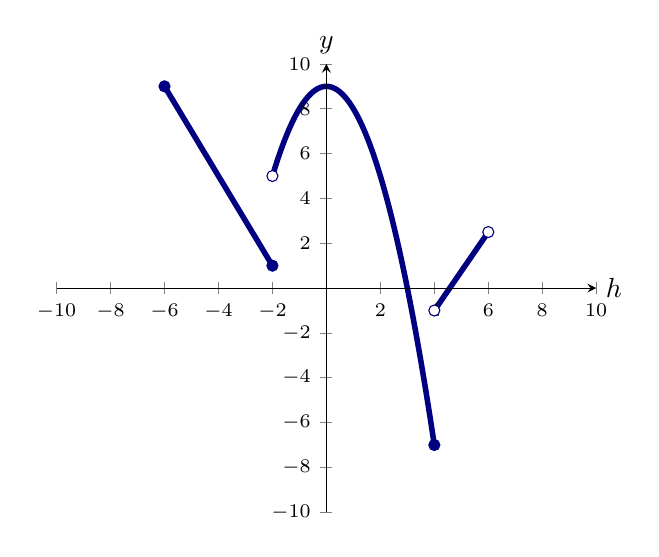
\begin{tikzpicture} 
  \begin{axis}[
            domain=-10:10, ymax=10, xmax=10, ymin=-10, xmin=-10,
            axis lines =center, xlabel=$h$, ylabel=$y$,
            ytick={-10,-8,-6,-4,-2,2,4,6,8,10},
            xtick={-10,-8,-6,-4,-2,2,4,6,8,10},
            ticklabel style={font=\scriptsize},
            every axis y label/.style={at=(current axis.above origin),anchor=south},
            every axis x label/.style={at=(current axis.right of origin),anchor=west},
            axis on top
          ]
          
      \addplot [line width=2, penColor, smooth,samples=100,domain=(-6:-2)] {-2*x-3};
          \addplot [line width=2, penColor, smooth,samples=100,domain=(-2:4)] {-1*(x+3)*(x-3))};
          \addplot [line width=2, penColor, smooth,samples=100,domain=(4:6)] {1.75*x-8};




      \addplot[color=penColor,fill=penColor,only marks,mark=*] coordinates{(-6,9)};
      \addplot[color=penColor,fill=penColor,only marks,mark=*] coordinates{(-2,1)};

      \addplot[color=penColor,fill=white,only marks,mark=*] coordinates{(-2,5)};
      \addplot[color=penColor,fill=penColor,only marks,mark=*] coordinates{(4,-7)};

      \addplot[color=penColor,fill=white,only marks,mark=*] coordinates{(4,-1)};
      \addplot[color=penColor,fill=white,only marks,mark=*] coordinates{(6,2.5)};


           

  \end{axis}
\end{tikzpicture}
\end{image}



From the graph, it appears that... \\

\begin{itemize}

\item The domain of $V$ is $[-6,6)$.
\item $V$ has a global maximum of $9$, which occurs at $\answer{-6}$ and at $\answer{0}$.
\item $V$ has a global minimum of $-7$, which occurs at $4$.
\item $V$ has a local minimum of $1$, which occurs at $-2$.
\item $V$ has a jump discontinuity at $-2$.
\item $V$ has a jump discontinuity at $4$.
\item $V$ is decreasing on $[-6, -2]$.
\item $V$ is increasing on $[-2, 0]$.
\item $V$ is decreasing on $\left[\answer{0}, \answer{4}\right]$.
\item $V$ is increasing on $[4, 6)$.


\end{itemize}








Let's define a new function based on $V$.\\





Let $f(x) = V(x)-2$ with the induced domain.

The domain of $f$ is $\left[\answer{-6}, \answer{6}\right)$, same as $V$. The range or function values $f$ are all $\answer{2}$ less than the function values of $V$.







\[
f(x) = 
\begin{cases}
  -2x-5 &  [-6, -2]   \\
  -(x+3)(x-3)-2 &  (-2, 4]  \\
  \frac{7x}{4} - 10 &  (4,6)
\end{cases}
\]












\begin{image}
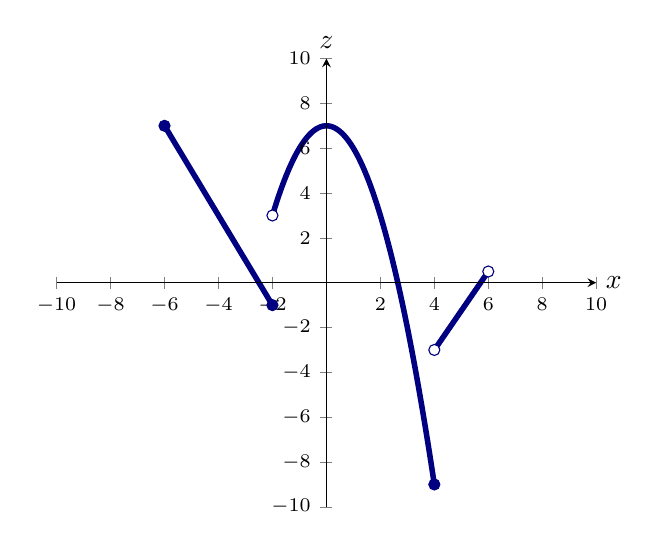
\begin{tikzpicture} 
  \begin{axis}[
            domain=-10:10, ymax=10, xmax=10, ymin=-10, xmin=-10,
            axis lines =center, xlabel=$x$, ylabel=$z$,
            ytick={-10,-8,-6,-4,-2,2,4,6,8,10},
            xtick={-10,-8,-6,-4,-2,2,4,6,8,10},
            ticklabel style={font=\scriptsize},
            every axis y label/.style={at=(current axis.above origin),anchor=south},
            every axis x label/.style={at=(current axis.right of origin),anchor=west},
            axis on top
          ]
          
      \addplot [line width=2, penColor, smooth,samples=100,domain=(-6:-2)] {-2*x-5};
          \addplot [line width=2, penColor, smooth,samples=100,domain=(-2:4)] {-1*(x+3)*(x-3))-2};
          \addplot [line width=2, penColor, smooth,samples=100,domain=(4:6)] {1.75*x-10};




      \addplot[color=penColor,fill=penColor,only marks,mark=*] coordinates{(-6,7)};
      \addplot[color=penColor,fill=penColor,only marks,mark=*] coordinates{(-2,-1)};

      \addplot[color=penColor,fill=white,only marks,mark=*] coordinates{(-2,3)};
      \addplot[color=penColor,fill=penColor,only marks,mark=*] coordinates{(4,-9)};

      \addplot[color=penColor,fill=white,only marks,mark=*] coordinates{(4,-3)};
      \addplot[color=penColor,fill=white,only marks,mark=*] coordinates{(6,0.5)};


           

  \end{axis}
\end{tikzpicture}
\end{image}





From the graph, it appears that... \\

\begin{itemize}

\item The domain of $f$ is $[-6,6)$.
\item $f$ has a global maximum of $7$, one of which occurs at $-6$ and the other occurs at $\answer{0}$.
\item $f$ has a global minimum of $-9$, which occurs at $4$.
\item $V$ has a local minimum of $-1$, which occurs at $-2$.
\item $f$ has a jump discontinuity at $-2$.
\item $f$ has a jump discontinuity at $4$.
\item $f$ is decreasing on $[-6, -2]$.
\item $f$ is increasing on $[-2, 0]$.
\item $f$ is decreasing on $\left[\answer{0}, \answer{4}\right]$.
\item $f$ is increasing on $[4, 6)$.


\end{itemize}



The places in the domain where characteristics and features occur did not changed.  The maximums and minimums have all dropped by $2$.  The endpoints are all still solid or hollow.  Their vertical coordinates have all dropped by $2$.






\end{example}


































































Let $X(y)$ be a function with its domain.

Let $P(r)$ be defined as $P(r) = X(r)-7$ with its induced domain.


Then the domain of $P$ is

\begin{multipleChoice}
\choice {the domain of $X$ shifted left $7$}
\choice {the domain of $X$ shifted right $7$}
\choice[correct] {the same as for $X$}
\end{multipleChoice}













\begin{example} Shifting Vertically




Graph of $y = m(f)$.

\begin{image}
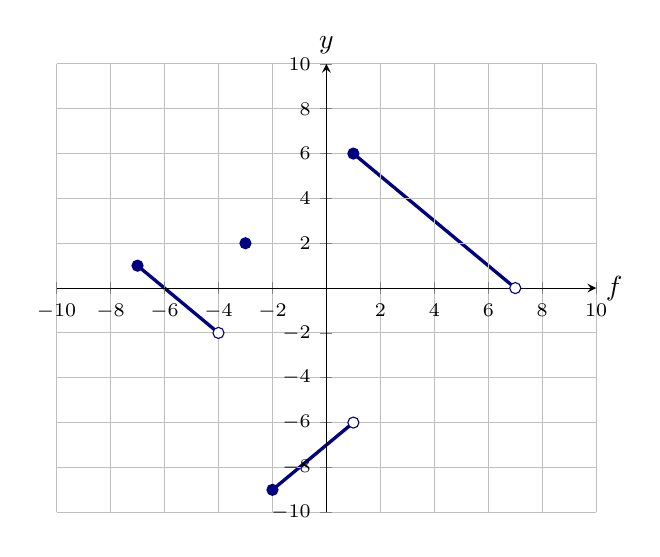
\begin{tikzpicture}
  \begin{axis}[
            domain=-10:10, ymax=10, xmax=10, ymin=-10, xmin=-10,
            axis lines =center, xlabel=$f$, ylabel=$y$, grid = major,
            ytick={-10,-8,-6,-4,-2,2,4,6,8,10},
            xtick={-10,-8,-6,-4,-2,2,4,6,8,10},
            ticklabel style={font=\scriptsize},
            every axis y label/.style={at=(current axis.above origin),anchor=south},
            every axis x label/.style={at=(current axis.right of origin),anchor=west},
            axis on top
          ]
          
  \addplot [draw=penColor,very thick,smooth,domain=(-7:-4)] {-x-6};
  \addplot [draw=penColor,very thick,smooth,domain=(-2:1)] {x-7};
  \addplot [draw=penColor,very thick,smooth,domain=(1:7)] {-x+7};

  \addplot[color=penColor,only marks,mark=*] coordinates{(-3,2)}; 
  
  \addplot[color=penColor,only marks,mark=*] coordinates{(-7,1)}; 
  \addplot[color=penColor,fill=white,only marks,mark=*] coordinates{(-4,-2)}; 
  \addplot[color=penColor,only marks,mark=*] coordinates{(-2,-9)}; 
  \addplot[color=penColor,fill=white,only marks,mark=*] coordinates{(1,-6)}; 
  \addplot[color=penColor,only marks,mark=*] coordinates{(1,6)}; 
  \addplot[color=penColor,fill=white,only marks,mark=*] coordinates{(7,0)}; 


    \end{axis}
\end{tikzpicture}
\end{image}








\begin{itemize}

\item The domain of $m$ is $[-7,-4) \cup \left\{\answer{-3}\right\} \cup [-2,7)$.
\item $m$ has a global (and local) maximum of $6$, which occurs at $\answer{1}$. 
\item $m$ has a global (and local) minimum of $-9$, which occurs at $\answer{-2}$. 
\item $m$ has a local maximum of $\answer{1}$, which occurs at $-7$.

\end{itemize}


$\answer{2}$ is both a local maximum and minimum of $m$.  \\

To see that $2$ is a local maximum at $-3$, imagine the interval $(-3.1, -2.9)$. For all of the domain elements in this interval, $T(-3)=2$ is the maximum.  This is automatically satisfied, since $3$ is the only domain element of $m$ inside this interval.  

\textbf{Note:} The definition of local maximum never promised that there would be other domain numbers in the small neighborhood.  It simply says that you need to supply an open interval around $-3$ such that $T(-3)$ is greater than or equal to all function values for all domain numbers inside the interval. \\

To see that $2$ is a local minimum, imagine the interval $(-3.1, -2.9)$. For all of the domain elements in this interval, $T(-3)=2$ is the minimum.  This is automatically satisfied, since $3$ is the only domain element of $m$ inside this interval.  


\textbf{Note:} The definition of local minimum never promised that there would be other domain numbers in the small neighborhood.  It simply says that you need to supply an open interval around $-3$ such that $T(-3)$ is less than or equal to all function values for all domain numbers inside the interval. \\




$\blacktriangleright$ Now, we'll shift the range. \\



Graph of $z = P(t) = m(t)+3$.

\begin{image}
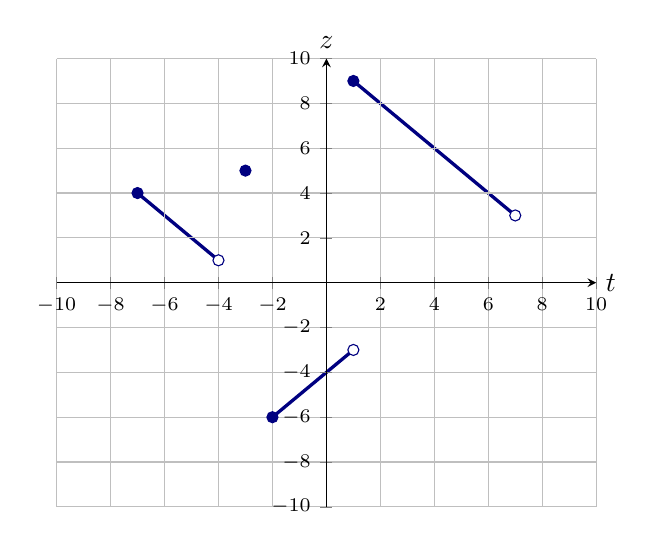
\begin{tikzpicture}
  \begin{axis}[
            domain=-10:10, ymax=10, xmax=10, ymin=-10, xmin=-10,
            axis lines =center, xlabel=$t$, ylabel=$z$, grid = major,
            ytick={-10,-8,-6,-4,-2,2,4,6,8,10},
            xtick={-10,-8,-6,-4,-2,2,4,6,8,10},
            ticklabel style={font=\scriptsize},
            every axis y label/.style={at=(current axis.above origin),anchor=south},
            every axis x label/.style={at=(current axis.right of origin),anchor=west},
            axis on top
          ]
          
  \addplot [draw=penColor,very thick,smooth,domain=(-7:-4)] {-x-3};
  \addplot [draw=penColor,very thick,smooth,domain=(-2:1)] {x-4};
  \addplot [draw=penColor,very thick,smooth,domain=(1:7)] {-x+10};

  \addplot[color=penColor,only marks,mark=*] coordinates{(-3,5)}; 
  
  \addplot[color=penColor,only marks,mark=*] coordinates{(-7,4)}; 
  \addplot[color=penColor,fill=white,only marks,mark=*] coordinates{(-4,1)}; 
  \addplot[color=penColor,only marks,mark=*] coordinates{(-2,-6)}; 
  \addplot[color=penColor,fill=white,only marks,mark=*] coordinates{(1,-3)}; 
  \addplot[color=penColor,only marks,mark=*] coordinates{(1,9)}; 
  \addplot[color=penColor,fill=white,only marks,mark=*] coordinates{(7,3)}; 


    \end{axis}
\end{tikzpicture}
\end{image}




\begin{itemize}

\item The domain of $P$ is $[-7,-4) \cup \{-3\} \cup [-2,7)$.
\item $P$ has a global (and local) maximum of $6+\answer{3}=9$, which occurs at $\answer{1}$. 
\item $P$ has a global (and local) minimum of $-9+\answer{3}=-6$, which occurs at $\answer{-2}$. 
\item $P$ has a local maximum of $1+\answer{3}=4$, which occurs at $\answer{-7}$.
\item $\answer{5}$ is both a local maximum and minimum of $P$ occuring at $-3$. 

\end{itemize}


\end{example}


















\begin{example} Sine



Graph of $y = \sin(\theta)$.

\begin{image}
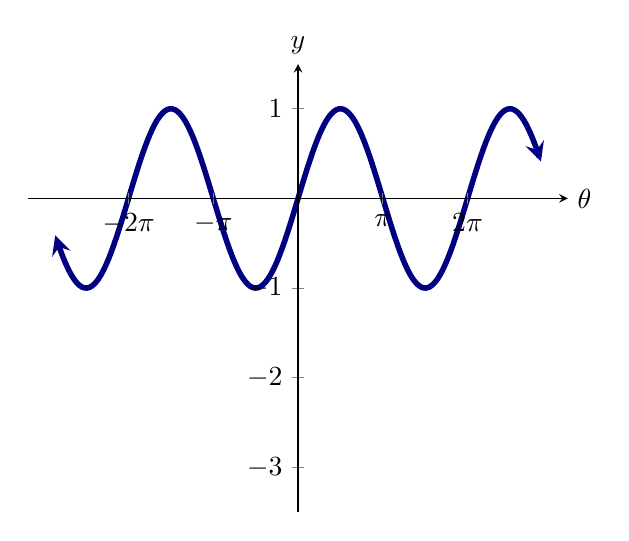
\begin{tikzpicture} 
  \begin{axis}[
            domain=-10:10, ymax=1.5, xmax=10, ymin=-3.5, xmin=-10,
            xtick={-6.28, -3.14, 3.14, 6.28}, 
            xticklabels={$-2\pi$, $-\pi$, $\pi$, $2\pi$},
            axis lines =center,  xlabel={$\theta$}, ylabel=$y$,
            every axis y label/.style={at=(current axis.above origin),anchor=south},
            every axis x label/.style={at=(current axis.right of origin),anchor=west},
            axis on top
          ]
          
            \addplot [line width=2, penColor, smooth,samples=200,domain=(-9:9), <->] {sin(deg(x))};

           

  \end{axis}
\end{tikzpicture}
\end{image}



\begin{itemize}
\item The zeros of $\sin(\theta)$ are all integer multiples of $\pi$.
\item The maximum value is $1$ and it occurs at:  $\left\{     \frac{(4k+1)\pi}{2} \, | \, k \in \textbf{Z}     \right\} = \{ \cdots, \frac{-3\pi}{2}, \frac{\pi}{2}, \frac{5\pi}{2}, \cdots \}$
\item The minimum value is $-1$ and it occurs at:  $\left\{    \frac{(4k+3)\pi}{2} \, | \, k \in \textbf{Z}     \right\} = \{ \cdots, \frac{-5\pi}{2}, \frac{-\pi}{2}, \frac{3\pi}{2}, \cdots \}$
\end{itemize}






Graph of $y = \sin(\theta) - 2$.

\begin{image}
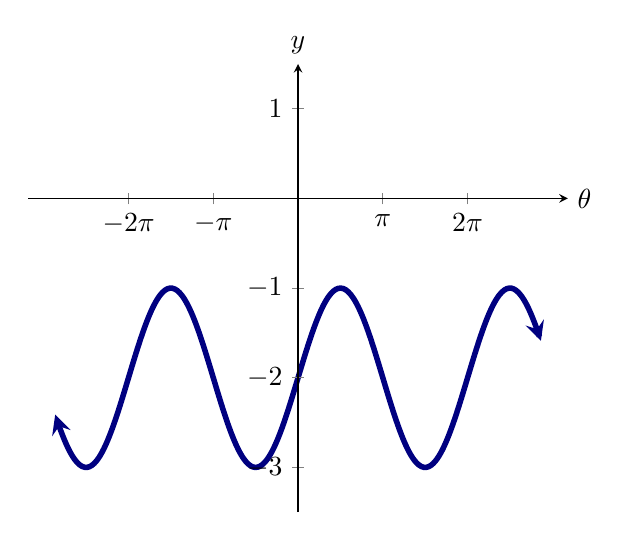
\begin{tikzpicture} 
  \begin{axis}[
            domain=-10:10, ymax=1.5, xmax=10, ymin=-3.5, xmin=-10,
            xtick={-6.28, -3.14, 3.14, 6.28}, 
            xticklabels={$-2\pi$, $-\pi$, $\pi$, $2\pi$},
            axis lines =center,  xlabel={$\theta$}, ylabel=$y$,
            every axis y label/.style={at=(current axis.above origin),anchor=south},
            every axis x label/.style={at=(current axis.right of origin),anchor=west},
            axis on top
          ]
          
            \addplot [line width=2, penColor, smooth,samples=200,domain=(-9:9), <->] {sin(deg(x))-2};

           

  \end{axis}
\end{tikzpicture}
\end{image}



\begin{itemize}
\item No zeros.
\item The maximum value is $-1$ and it occurs at:  $\left\{     \frac{(4k+1)\pi}{2} \, | \, k \in \textbf{Z}     \right\}$
\item The minimum value is $-3$ and it occurs at:  $\left\{    \frac{(4k+3)\pi}{2} \, | \, k \in \textbf{Z}     \right\}$
\end{itemize}














\end{example}






Adding or subtracting a constant from the function, as opposed to the domain, shifts the graph up and down.  The shape of the graph doesn't change.  All of the characteristics and features of the function, like maximums and minimums, occur at the same places in the domain.  Their values just change accordingly.



























\subsection*{Together}

We can apply horizontal and vertical shifts together as well.





\begin{example}  Shifting

Let $B(r) = |r-3| + 2$.  \\


We have shifted the absolute value function to the \wordChoice{\choice{left} \choice[correct]{right}} by \wordChoice{\choice{-3} \choice{-2} \choice{2} \choice[correct]{3}} and \wordChoice{\choice[correct]{up} \choice{down}}  by \wordChoice{\choice[correct]{2} \choice{3}}.


\begin{image}
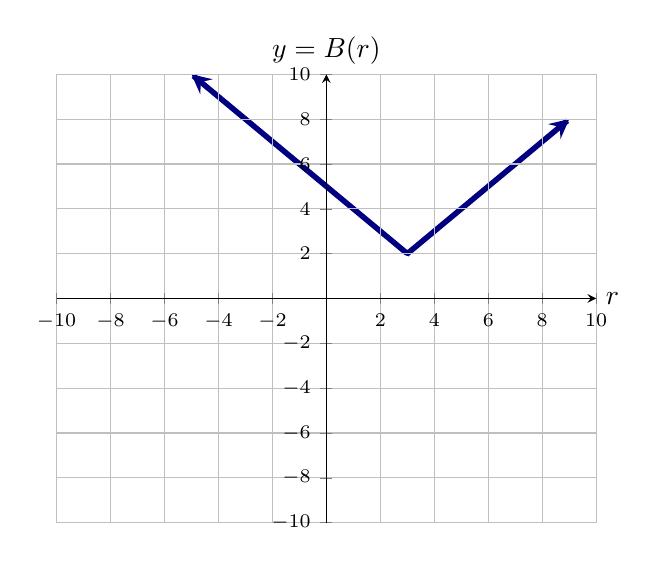
\begin{tikzpicture} 
  \begin{axis}[
            domain=-10:10, ymax=10, xmax=10, ymin=-10, xmin=-10,
            axis lines =center, xlabel=$r$, ylabel={$y=B(r)$}, grid = major,
            ytick={-10,-8,-6,-4,-2,2,4,6,8,10},
            xtick={-10,-8,-6,-4,-2,2,4,6,8,10},
            ticklabel style={font=\scriptsize},
            every axis y label/.style={at=(current axis.above origin),anchor=south},
            every axis x label/.style={at=(current axis.right of origin),anchor=west},
            axis on top
          ]
          
          \addplot [line width=2, penColor, smooth, samples=200, domain=(-5:9),<->] {abs(x-3)+2};
        

  \end{axis}
\end{tikzpicture}
\end{image}




The graph of the absolute value function looks like a ``V'', which is also the shape of the graph of $B$. \\


The graph of the absolute value function has a corner at $(0, 0)$.  The corner in the graph of $B$ is now at $(3, 2)$. \\

Another way of saying this is that the absolute value function, $A(t) = |t|$ has a global minimum of $0$ at $0$.  This minimum occurs when the inside of the vertical bars equals $0$.

For $B$, this happens when $r-3=0$. $r=\answer{3}$.



\end{example}

































\begin{center}
\textbf{\textcolor{green!50!black}{oooo-=-=-=-ooOoo-=-=-=-ooooo}} \\

more examples can be found by following this link\\ \link[More Examples of Shifting]{https://ximera.osu.edu/csccmathematics/precalculus/precalculus/transformations/examples/exampleList}

\end{center}







\end{document}
